%%%%%%%%%%%%%%%%%%%%%%%%%%%%%%%%%%%%%%%%%%%%%%%%%%%%%%%%%%%%%%%%%%%%%%%%%%%%%%%%
% CHAPTER 6
%%%%%%%%%%%%%%%%%%%%%%%%%%%%%%%%%%%%%%%%%%%%%%%%%%%%%%%%%%%%%%%%%%%%%%%%%%%%%%%%

\chapter{Sampling Theorem and Reconstruction}

\begin{tcolorbox}[colback=blue!5!white,colframe=blue!70!black,title=Learning Objectives]

After studying this chapter, the reader will be able to

\begin{itemize}
\item Understand the need for sampling.
\item Define sampling frequency and sampling period.
\item State and prove the Nyquist sampling theorem.
\item Explain aliasing and spectral overlap.
\item Determine the minimum sampling rate for a given signal.
\item Understand ideal reconstruction using a low-pass filter.
\end{itemize}

\end{tcolorbox}

%%%%%%%%%%%%%%%%%%%%%%%%%%%%%%%%%%%%%%%%%%%%%%%%%%%%%%%%%%%%%%%%%%%%%%%%%%%%%%%%

\section{Introduction}

Real-world signals such as speech, ECG, seismic data and sensor outputs are
continuous-time signals. Digital systems, however, can process only discrete-time
samples.

The process of converting a continuous-time signal into a sequence of samples is
called \textbf{sampling}.

\begin{center}
\begin{tikzpicture}[node distance=2.5cm,>=Latex]
\node[draw,minimum width=2.8cm,minimum height=1cm] (x) {Continuous signal $x(t)$};
\node[draw,minimum width=2.2cm,minimum height=1cm,right of=x] (s) {Sampler};
\node[draw,minimum width=3cm,minimum height=1cm,right of=s] (xs) {Samples $x[n]$};

\draw[->] (x) -- (s);
\draw[->] (s) -- (xs);
\end{tikzpicture}
\end{center}

The central question is:

\begin{center}
\textbf{How fast should we sample a signal so that it can be perfectly reconstructed?}
\end{center}

%%%%%%%%%%%%%%%%%%%%%%%%%%%%%%%%%%%%%%%%%%%%%%%%%%%%%%%%%%%%%%%%%%%%%%%%%%%%%%%%

\section{Sampling Period and Sampling Frequency}

Let

\[
T_s=\text{sampling period (seconds)}
\]

\[
f_s=\text{sampling frequency (samples/second)}
\]

They are related by

\[
\boxed{
f_s=\frac{1}{T_s}
}
\]

%%%%%%%%%%%%%%%%%%%%%%%%%%%%%%%%%%%%%%%%%%%%%%%%%%%%%%%%%%%%%%%%%%%%%%%%%%%%%%%%

\subsection{Example}

If

\[
T_s=1\text{ ms}=10^{-3}\text{ s},
\]

then

\[
f_s=\frac{1}{10^{-3}}=1000\text{ Hz}=1\text{ kHz}.
\]

%%%%%%%%%%%%%%%%%%%%%%%%%%%%%%%%%%%%%%%%%%%%%%%%%%%%%%%%%%%%%%%%%%%%%%%%%%%%%%%%

\section{Discrete-Time Sequence}

Sampling a continuous-time signal at instants

\[
t=nT_s,\qquad n=0,\pm1,\pm2,\ldots
\]

produces the discrete sequence

\[
\boxed{
x[n]=x(nT_s)
}
\]

%%%%%%%%%%%%%%%%%%%%%%%%%%%%%%%%%%%%%%%%%%%%%%%%%%%%%%%%%%%%%%%%%%%%%%%%%%%%%%%%

\section{Impulse Sampling}

Ideal sampling is modeled by multiplying the signal with an impulse train.

%%%%%%%%%%%%%%%%%%%%%%%%%%%%%%%%%%%%%%%%%%%%%%%%%%%%%%%%%%%%%%%%%%%%%%%%%%%%%%%%

\subsection{Impulse Train}

\[
\boxed{
p(t)=\sum_{n=-\infty}^{\infty}\delta(t-nT_s)
}
\]

%%%%%%%%%%%%%%%%%%%%%%%%%%%%%%%%%%%%%%%%%%%%%%%%%%%%%%%%%%%%%%%%%%%%%%%%%%%%%%%%

\subsection{Sampled Signal}

\[
x_s(t)=x(t)p(t)
\]

Substituting \(p(t)\),

\[
\boxed{
x_s(t)=
\sum_{n=-\infty}^{\infty}
x(nT_s)\delta(t-nT_s)
}
\]

Thus, the amplitudes of the impulses are the sample values.

%%%%%%%%%%%%%%%%%%%%%%%%%%%%%%%%%%%%%%%%%%%%%%%%%%%%%%%%%%%%%%%%%%%%%%%%%%%%%%%%

\section{Spectrum of the Impulse Train}

The Fourier transform of the impulse train is another impulse train:

\[
\boxed{
P(\omega)=
\frac{2\pi}{T_s}
\sum_{k=-\infty}^{\infty}
\delta(\omega-k\omega_s)
}
\]

where

\[
\boxed{
\omega_s=\frac{2\pi}{T_s}=2\pi f_s
}
\]

is the sampling angular frequency.

%%%%%%%%%%%%%%%%%%%%%%%%%%%%%%%%%%%%%%%%%%%%%%%%%%%%%%%%%%%%%%%%%%%%%%%%%%%%%%%%

\section{Spectrum of the Sampled Signal}

Since multiplication in time corresponds to convolution in frequency,

\[
X_s(\omega)=
\frac{1}{2\pi}
X(\omega)*P(\omega)
\]

Substituting \(P(\omega)\),

\[
\boxed{
X_s(\omega)=
\frac{1}{T_s}
\sum_{k=-\infty}^{\infty}
X(\omega-k\omega_s)
}
\]

%%%%%%%%%%%%%%%%%%%%%%%%%%%%%%%%%%%%%%%%%%%%%%%%%%%%%%%%%%%%%%%%%%%%%%%%%%%%%%%%

\subsection{Interpretation}

The original spectrum is repeated at

\[
\omega=0,\pm\omega_s,\pm2\omega_s,\ldots
\]

with spacing \(\omega_s\).

%%%%%%%%%%%%%%%%%%%%%%%%%%%%%%%%%%%%%%%%%%%%%%%%%%%%%%%%%%%%%%%%%%%%%%%%%%%%%%%%

\section{Bandlimited Signal}

A signal is bandlimited if

\[
\boxed{
X(\omega)=0,\qquad |\omega|>\omega_m
}
\]

where \(\omega_m\) is the highest frequency present.

Equivalently, in hertz,

\[
f_m=\frac{\omega_m}{2\pi}.
\]

%%%%%%%%%%%%%%%%%%%%%%%%%%%%%%%%%%%%%%%%%%%%%%%%%%%%%%%%%%%%%%%%%%%%%%%%%%%%%%%%

\section{Sampling Theorem}

\begin{tcolorbox}[title=Nyquist Sampling Theorem,colback=yellow!10]

A bandlimited signal with maximum frequency \(f_m\) can be perfectly reconstructed
from its samples if the sampling frequency satisfies

\[
\boxed{
f_s\ge 2f_m
}
\]

The minimum sampling frequency

\[
\boxed{
f_N=2f_m
}
\]

is called the \textbf{Nyquist rate}.

\end{tcolorbox}

%%%%%%%%%%%%%%%%%%%%%%%%%%%%%%%%%%%%%%%%%%%%%%%%%%%%%%%%%%%%%%%%%%%%%%%%%%%%%%%%

\section{Why \(2f_m\)?}

The original spectrum occupies

\[
-f_m\le f\le f_m.
\]

After sampling, copies appear centered at \(\pm f_s\).

To avoid overlap,

\[
f_s-f_m\ge f_m
\]

which gives

\[
\boxed{
f_s\ge2f_m
}
\]

%%%%%%%%%%%%%%%%%%%%%%%%%%%%%%%%%%%%%%%%%%%%%%%%%%%%%%%%%%%%%%%%%%%%%%%%%%%%%%%%

\section{Case 1: Proper Sampling}

If

\[
f_s>2f_m,
\]

the spectral copies are separated.

\begin{center}
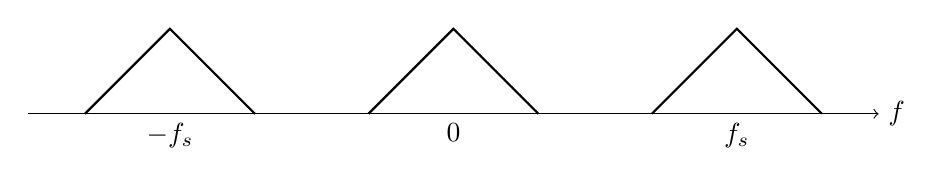
\begin{tikzpicture}[scale=0.9]
\draw[->] (-6,0) -- (6,0) node[right] {$f$};

\draw[thick] (-1.2,0) -- (0,1.2) -- (1.2,0);

\draw[thick] (-5.2,0) -- (-4,1.2) -- (-2.8,0);

\draw[thick] (2.8,0) -- (4,1.2) -- (5.2,0);

\node[below] at (0,0) {$0$};
\node[below] at (4,0) {$f_s$};
\node[below] at (-4,0) {$-f_s$};
\end{tikzpicture}
\end{center}

Perfect reconstruction is possible.

%%%%%%%%%%%%%%%%%%%%%%%%%%%%%%%%%%%%%%%%%%%%%%%%%%%%%%%%%%%%%%%%%%%%%%%%%%%%%%%%

\section{Case 2: Critical Sampling}

If

\[
f_s=2f_m,
\]

the spectra just touch.

This is the theoretical minimum rate.

%%%%%%%%%%%%%%%%%%%%%%%%%%%%%%%%%%%%%%%%%%%%%%%%%%%%%%%%%%%%%%%%%%%%%%%%%%%%%%%%

\section{Case 3: Undersampling}

If

\[
f_s<2f_m,
\]

the spectra overlap.

\begin{center}
\begin{tikzpicture}[scale=0.9]
\draw[->] (-5,0) -- (5,0) node[right] {$f$};

\draw[thick] (-2.2,0) -- (-1,1.2) -- (0.2,0);

\draw[thick] (-0.2,0) -- (1,1.2) -- (2.2,0);

\node[below] at (0,0) {$0$};
\end{tikzpicture}
\end{center}

This phenomenon is called \textbf{aliasing}.

%%%%%%%%%%%%%%%%%%%%%%%%%%%%%%%%%%%%%%%%%%%%%%%%%%%%%%%%%%%%%%%%%%%%%%%%%%%%%%%%

\section{Aliasing}

\subsection{Definition}

Aliasing occurs when different frequency components become indistinguishable after
sampling.

%%%%%%%%%%%%%%%%%%%%%%%%%%%%%%%%%%%%%%%%%%%%%%%%%%%%%%%%%%%%%%%%%%%%%%%%%%%%%%%%

\subsection{Alias Frequency Formula}

For a sinusoid of frequency \(f\),

\[
\boxed{
f_a=\left|f-kf_s\right|
}
\]

where \(k\) is chosen so that \(0\le f_a\le f_s/2\).

%%%%%%%%%%%%%%%%%%%%%%%%%%%%%%%%%%%%%%%%%%%%%%%%%%%%%%%%%%%%%%%%%%%%%%%%%%%%%%%%

\subsection{Example}

Let

\[
f=900\text{ Hz},
\qquad
f_s=1000\text{ Hz}.
\]

Choose \(k=1\):

\[
f_a=|900-1000|=100\text{ Hz}.
\]

So a 900 Hz signal appears as a 100 Hz signal after sampling.

%%%%%%%%%%%%%%%%%%%%%%%%%%%%%%%%%%%%%%%%%%%%%%%%%%%%%%%%%%%%%%%%%%%%%%%%%%%%%%%%

\section{Nyquist Frequency}

The highest frequency that can be represented without aliasing is

\[
\boxed{
f_{max}=\frac{f_s}{2}
}
\]

called the \textbf{Nyquist frequency}.

%%%%%%%%%%%%%%%%%%%%%%%%%%%%%%%%%%%%%%%%%%%%%%%%%%%%%%%%%%%%%%%%%%%%%%%%%%%%%%%%

\section{Anti-Aliasing Filter}

Before sampling, the signal is passed through a low-pass filter to remove frequency
components above \(f_s/2\).

\begin{center}
\begin{tikzpicture}[node distance=2.2cm,>=Latex]
\node[draw,minimum width=2.2cm,minimum height=0.9cm] (x) {$x(t)$};
\node[draw,minimum width=2.8cm,minimum height=0.9cm,right of=x] (lpf) {Anti-alias LPF};
\node[draw,minimum width=2cm,minimum height=0.9cm,right of=lpf] (s) {Sampler};

\draw[->] (x) -- (lpf);
\draw[->] (lpf) -- (s);
\end{tikzpicture}
\end{center}

%%%%%%%%%%%%%%%%%%%%%%%%%%%%%%%%%%%%%%%%%%%%%%%%%%%%%%%%%%%%%%%%%%%%%%%%%%%%%%%%

\section{Ideal Reconstruction}

If \(f_s\ge2f_m\), the original signal can be recovered by an ideal low-pass filter.

%%%%%%%%%%%%%%%%%%%%%%%%%%%%%%%%%%%%%%%%%%%%%%%%%%%%%%%%%%%%%%%%%%%%%%%%%%%%%%%%

\subsection{Reconstruction Filter}

\[
\boxed{
H_r(\omega)=
\begin{cases}
T_s, & |\omega|\le\omega_m\\
0, & |\omega|>\omega_m
\end{cases}
}
\]

The filter passes the baseband copy and rejects all other spectral replicas.

%%%%%%%%%%%%%%%%%%%%%%%%%%%%%%%%%%%%%%%%%%%%%%%%%%%%%%%%%%%%%%%%%%%%%%%%%%%%%%%%

\section{Reconstruction Formula}

The reconstructed signal is

\[
x(t)=
\sum_{n=-\infty}^{\infty}
x(nT_s)\,
\mathrm{sinc}\left(\frac{t-nT_s}{T_s}\right)
\]

where

\[
\boxed{
\mathrm{sinc}(x)=\frac{\sin(\pi x)}{\pi x}
}
\]

This is the \textbf{sinc interpolation formula}.

%%%%%%%%%%%%%%%%%%%%%%%%%%%%%%%%%%%%%%%%%%%%%%%%%%%%%%%%%%%%%%%%%%%%%%%%%%%%%%%%

\section{Worked Example 6.1}

A signal contains frequencies up to

\[
f_m=5\text{ kHz}.
\]

Find the Nyquist rate and the minimum sampling period.

%%%%%%%%%%%%%%%%%%%%%%%%%%%%%%%%%%%%%%%%%%%%%%%%%%%%%%%%%%%%%%%%%%%%%%%%%%%%%%%%

\subsection{Solution}

\[
f_N=2f_m=10\text{ kHz}
\]

\[
T_s=\frac{1}{f_N}
=\frac{1}{10^4}
=100\ \mu s
\]

\[
\boxed{
f_N=10\text{ kHz},
\qquad
T_s=100\ \mu s
}
\]

%%%%%%%%%%%%%%%%%%%%%%%%%%%%%%%%%%%%%%%%%%%%%%%%%%%%%%%%%%%%%%%%%%%%%%%%%%%%%%%%

\section{Worked Example 6.2}

A signal is sampled at

\[
f_s=8\text{ kHz}.
\]

What is the maximum frequency that can be represented without aliasing?

%%%%%%%%%%%%%%%%%%%%%%%%%%%%%%%%%%%%%%%%%%%%%%%%%%%%%%%%%%%%%%%%%%%%%%%%%%%%%%%%

\subsection{Solution}

\[
f_{max}=\frac{f_s}{2}=4\text{ kHz}
\]

\[
\boxed{
f_{max}=4\text{ kHz}
}
\]

%%%%%%%%%%%%%%%%%%%%%%%%%%%%%%%%%%%%%%%%%%%%%%%%%%%%%%%%%%%%%%%%%%%%%%%%%%%%%%%%

\section{Worked Example 6.3}

A 6 kHz sinusoid is sampled at 8 kHz. Find the alias frequency.

%%%%%%%%%%%%%%%%%%%%%%%%%%%%%%%%%%%%%%%%%%%%%%%%%%%%%%%%%%%%%%%%%%%%%%%%%%%%%%%%

\subsection{Solution}

\[
f_a=|6-8|=2\text{ kHz}
\]

\[
\boxed{
f_a=2\text{ kHz}
}
\]

%%%%%%%%%%%%%%%%%%%%%%%%%%%%%%%%%%%%%%%%%%%%%%%%%%%%%%%%%%%%%%%%%%%%%%%%%%%%%%%%

\begin{tcolorbox}[title=Quick Recall,colback=blue!5]

\[
f_s=\frac{1}{T_s}
\]

\[
\omega_s=2\pi f_s
\]

\[
X_s(\omega)=
\frac{1}{T_s}
\sum_{k=-\infty}^{\infty}
X(\omega-k\omega_s)
\]

\[
f_s\ge2f_m
\]

\[
f_N=2f_m
\]

\[
f_{max}=\frac{f_s}{2}
\]

\[
f_a=|f-kf_s|
\]

\[
x(t)=
\sum_{n=-\infty}^{\infty}
x(nT_s)\,
\mathrm{sinc}\left(\frac{t-nT_s}{T_s}\right)
\]

\end{tcolorbox}
%%%%%%%%%%%%%%%%%%%%%%%%%%%%%%%%%%%%%%%%%%%%%%%%%%%%%%%%%%%%%%%%%%%%%%%%%%%%%%%%
%%%%%%%%%%%%%%%%%%%%%%%%%%%%%%%%%%%%%%%%%%%%%%%%%%%%%%%%%%%%%%%%%%%%%%%%%%%%%%%%
\section{Proof of the Sampling Theorem}

Assume \(x(t)\) is bandlimited:

\[
X(\omega)=0,\qquad |\omega|>\omega_m
\]

After sampling,

\[
X_s(\omega)=
\frac{1}{T_s}
\sum_{k=-\infty}^{\infty}
X(\omega-k\omega_s)
\]

The replicas are centered at

\[
0,\pm\omega_s,\pm2\omega_s,\ldots
\]

For perfect reconstruction, adjacent replicas must not overlap.

%%%%%%%%%%%%%%%%%%%%%%%%%%%%%%%%%%%%%%%%%%%%%%%%%%%%%%%%%%%%%%%%%%%%%%%%%%%%%%%%

\subsection{Condition}

The right edge of the baseband spectrum is \(\omega_m\).

The left edge of the first shifted replica is \(\omega_s-\omega_m\).

Require

\[
\omega_s-\omega_m\ge\omega_m
\]

Hence,

\[
\boxed{
\omega_s\ge2\omega_m
}
\]

Dividing by \(2\pi\),

\[
\boxed{
f_s\ge2f_m
}
\]

Thus, the Nyquist theorem is proved.

%%%%%%%%%%%%%%%%%%%%%%%%%%%%%%%%%%%%%%%%%%%%%%%%%%%%%%%%%%%%%%%%%%%%%%%%%%%%%%%%

\section{Natural Sampling}

In natural sampling, the switch remains ON for a short duration \(\tau\).

%%%%%%%%%%%%%%%%%%%%%%%%%%%%%%%%%%%%%%%%%%%%%%%%%%%%%%%%%%%%%%%%%%%%%%%%%%%%%%%%

\subsection{Waveform}

\begin{center}
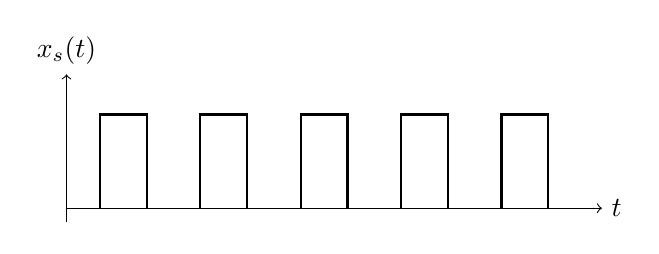
\begin{tikzpicture}[scale=0.85]
\draw[->] (0,0) -- (8,0) node[right] {$t$};
\draw[->] (0,-0.2) -- (0,2) node[above] {$x_s(t)$};

\foreach \x in {0.5,2,3.5,5,6.5}{
  \draw[thick] (\x,0) -- (\x,1.4) -- ++(0.7,0) -- ++(0,-1.4);
}
\end{tikzpicture}
\end{center}

The top of each pulse follows the original signal shape.

%%%%%%%%%%%%%%%%%%%%%%%%%%%%%%%%%%%%%%%%%%%%%%%%%%%%%%%%%%%%%%%%%%%%%%%%%%%%%%%%

\section{Flat-Top Sampling}

In practical sample-and-hold circuits, the sampled value is held constant during the pulse width.

%%%%%%%%%%%%%%%%%%%%%%%%%%%%%%%%%%%%%%%%%%%%%%%%%%%%%%%%%%%%%%%%%%%%%%%%%%%%%%%%

\subsection{Waveform}

\begin{center}
\begin{tikzpicture}[scale=0.85]
\draw[->] (0,0) -- (8,0) node[right] {$t$};
\draw[->] (0,-0.2) -- (0,2) node[above] {$x_s(t)$};

\draw[thick] (0.5,0) -- (0.5,0.8) -- (1.2,0.8) -- (1.2,0);
\draw[thick] (2,0) -- (2,1.3) -- (2.7,1.3) -- (2.7,0);
\draw[thick] (3.5,0) -- (3.5,0.6) -- (4.2,0.6) -- (4.2,0);
\draw[thick] (5,0) -- (5,1.5) -- (5.7,1.5) -- (5.7,0);
\end{tikzpicture}
\end{center}

This is the most common practical sampling method.

%%%%%%%%%%%%%%%%%%%%%%%%%%%%%%%%%%%%%%%%%%%%%%%%%%%%%%%%%%%%%%%%%%%%%%%%%%%%%%%%

\section{Aperture Effect}

Because the sample is averaged over a finite pulse width \(\tau\), high-frequency
components are attenuated.

%%%%%%%%%%%%%%%%%%%%%%%%%%%%%%%%%%%%%%%%%%%%%%%%%%%%%%%%%%%%%%%%%%%%%%%%%%%%%%%%

\subsection{Frequency Response}

\[
\boxed{
H_a(\omega)=
\tau\,\mathrm{sinc}\left(\frac{\omega\tau}{2}\right)
e^{-j\omega\tau/2}
}
\]

The magnitude response is

\[
|H_a(\omega)|=
\tau\left|
\mathrm{sinc}\left(\frac{\omega\tau}{2}\right)
\right|
\]

%%%%%%%%%%%%%%%%%%%%%%%%%%%%%%%%%%%%%%%%%%%%%%%%%%%%%%%%%%%%%%%%%%%%%%%%%%%%%%%%

\subsection{Consequence}

\begin{itemize}
\item Low frequencies are almost unaffected.
\item High frequencies are attenuated.
\item This produces amplitude distortion.
\end{itemize}

%%%%%%%%%%%%%%%%%%%%%%%%%%%%%%%%%%%%%%%%%%%%%%%%%%%%%%%%%%%%%%%%%%%%%%%%%%%%%%%%

\section{Oversampling}

Oversampling means

\[
\boxed{
f_s\gg2f_m
}
\]

%%%%%%%%%%%%%%%%%%%%%%%%%%%%%%%%%%%%%%%%%%%%%%%%%%%%%%%%%%%%%%%%%%%%%%%%%%%%%%%%

\subsection{Advantages}

\begin{itemize}
\item Easier anti-aliasing filter design.
\item Reduced quantization noise in the signal band.
\item Better signal-to-noise ratio after digital filtering.
\end{itemize}

%%%%%%%%%%%%%%%%%%%%%%%%%%%%%%%%%%%%%%%%%%%%%%%%%%%%%%%%%%%%%%%%%%%%%%%%%%%%%%%%

\subsection{Example}

Audio signals are often sampled at

\[
44.1\text{ kHz}
\]

even though human hearing is limited to about

\[
20\text{ kHz}.
\]

%%%%%%%%%%%%%%%%%%%%%%%%%%%%%%%%%%%%%%%%%%%%%%%%%%%%%%%%%%%%%%%%%%%%%%%%%%%%%%%%

\section{Undersampling}

If

\[
f_s<2f_m,
\]

aliasing occurs.

%%%%%%%%%%%%%%%%%%%%%%%%%%%%%%%%%%%%%%%%%%%%%%%%%%%%%%%%%%%%%%%%%%%%%%%%%%%%%%%%

\subsection{Example}

A 7 kHz signal sampled at 10 kHz gives

\[
f_a=|7-10|=3\text{ kHz}
\]

The reconstructed signal contains a false 3 kHz component.

%%%%%%%%%%%%%%%%%%%%%%%%%%%%%%%%%%%%%%%%%%%%%%%%%%%%%%%%%%%%%%%%%%%%%%%%%%%%%%%%

\section{Bandpass Sampling}

If a signal occupies a band

\[
f_L\le f\le f_H,
\]

it is sometimes possible to sample below \(2f_H\).

%%%%%%%%%%%%%%%%%%%%%%%%%%%%%%%%%%%%%%%%%%%%%%%%%%%%%%%%%%%%%%%%%%%%%%%%%%%%%%%%

\subsection{Condition}

For an integer \(n\),

\[
\boxed{
\frac{2f_H}{n}
\le
f_s
\le
\frac{2f_L}{n-1}
}
\]

This technique is widely used in radio receivers.

%%%%%%%%%%%%%%%%%%%%%%%%%%%%%%%%%%%%%%%%%%%%%%%%%%%%%%%%%%%%%%%%%%%%%%%%%%%%%%%%

\section{Example of Bandpass Sampling}

Suppose

\[
f_L=90\text{ MHz},
\qquad
f_H=100\text{ MHz}.
\]

The signal bandwidth is

\[
B=10\text{ MHz}.
\]

Instead of sampling at

\[
200\text{ MHz},
\]

a suitable lower sampling frequency can be chosen using the bandpass sampling
condition.

%%%%%%%%%%%%%%%%%%%%%%%%%%%%%%%%%%%%%%%%%%%%%%%%%%%%%%%%%%%%%%%%%%%%%%%%%%%%%%%%

\section{Reconstruction Filter}

The ideal reconstruction filter has cutoff

\[
\omega_c=\omega_m.
\]

Its frequency response is

\[
H_r(\omega)=
\begin{cases}
T_s, & |\omega|\le\omega_m\\
0, & |\omega|>\omega_m
\end{cases}
\]

%%%%%%%%%%%%%%%%%%%%%%%%%%%%%%%%%%%%%%%%%%%%%%%%%%%%%%%%%%%%%%%%%%%%%%%%%%%%%%%%

\subsection{Why Gain \(T_s\)?}

The sampled spectrum is scaled by \(1/T_s\).

The reconstruction filter multiplies it by \(T_s\), restoring the original amplitude.

%%%%%%%%%%%%%%%%%%%%%%%%%%%%%%%%%%%%%%%%%%%%%%%%%%%%%%%%%%%%%%%%%%%%%%%%%%%%%%%%

\section{Sinc Interpolation}

The reconstructed signal is

\[
\boxed{
x(t)=
\sum_{n=-\infty}^{\infty}
x(nT_s)\,
\mathrm{sinc}\left(\frac{t-nT_s}{T_s}\right)
}
\]

Each sample generates a shifted sinc pulse, and the sum of all sinc pulses
reconstructs the original signal exactly.

%%%%%%%%%%%%%%%%%%%%%%%%%%%%%%%%%%%%%%%%%%%%%%%%%%%%%%%%%%%%%%%%%%%%%%%%%%%%%%%%

\section{Why Sinc Passes Through the Samples}

Since

\[
\mathrm{sinc}(0)=1
\]

and

\[
\mathrm{sinc}(k)=0,\qquad k=\pm1,\pm2,\ldots
\]

at \(t=mT_s\),

\[
x(mT_s)=x[m].
\]

Thus, the interpolation passes through every sample point.

%%%%%%%%%%%%%%%%%%%%%%%%%%%%%%%%%%%%%%%%%%%%%%%%%%%%%%%%%%%%%%%%%%%%%%%%%%%%%%%%

\section{Solved Example 6.4}

A signal has maximum frequency

\[
f_m=12\text{ kHz}.
\]

Find the Nyquist rate, minimum sampling period, and a practical sampling frequency.

%%%%%%%%%%%%%%%%%%%%%%%%%%%%%%%%%%%%%%%%%%%%%%%%%%%%%%%%%%%%%%%%%%%%%%%%%%%%%%%%

\subsection{Solution}

Nyquist rate:

\[
f_N=2f_m=24\text{ kHz}
\]

Minimum sampling period:

\[
T_s=\frac{1}{24\times10^3}=41.67\ \mu s
\]

A practical choice is

\[
\boxed{
f_s=30\text{ kHz}
}
\]

%%%%%%%%%%%%%%%%%%%%%%%%%%%%%%%%%%%%%%%%%%%%%%%%%%%%%%%%%%%%%%%%%%%%%%%%%%%%%%%%

\section{Solved Example 6.5}

A 15 kHz signal is sampled at 20 kHz. Determine the alias frequency.

%%%%%%%%%%%%%%%%%%%%%%%%%%%%%%%%%%%%%%%%%%%%%%%%%%%%%%%%%%%%%%%%%%%%%%%%%%%%%%%%

\subsection{Solution}

\[
f_a=|15-20|=5\text{ kHz}
\]

\[
\boxed{
f_a=5\text{ kHz}
}
\]

%%%%%%%%%%%%%%%%%%%%%%%%%%%%%%%%%%%%%%%%%%%%%%%%%%%%%%%%%%%%%%%%%%%%%%%%%%%%%%%%

\section{Solved Example 6.6}

A signal contains frequencies up to 3 kHz and is sampled at 6 kHz. Is perfect
reconstruction possible?

%%%%%%%%%%%%%%%%%%%%%%%%%%%%%%%%%%%%%%%%%%%%%%%%%%%%%%%%%%%%%%%%%%%%%%%%%%%%%%%%

\subsection{Solution}

\[
f_s=6\text{ kHz},
\qquad
2f_m=6\text{ kHz}
\]

Since

\[
f_s=2f_m,
\]

the signal is sampled at the Nyquist rate.

\[
\boxed{
\text{Yes, perfect reconstruction is theoretically possible.}
}
\]

In practice, a slightly higher sampling frequency is preferred.

%%%%%%%%%%%%%%%%%%%%%%%%%%%%%%%%%%%%%%%%%%%%%%%%%%%%%%%%%%%%%%%%%%%%%%%%%%%%%%%%

\section{Solved Example 6.7}

A signal is sampled at 48 kHz. What is the Nyquist frequency?

%%%%%%%%%%%%%%%%%%%%%%%%%%%%%%%%%%%%%%%%%%%%%%%%%%%%%%%%%%%%%%%%%%%%%%%%%%%%%%%%

\subsection{Solution}

\[
f_N=\frac{48}{2}=24\text{ kHz}
\]

\[
\boxed{
f_N=24\text{ kHz}
}
\]

%%%%%%%%%%%%%%%%%%%%%%%%%%%%%%%%%%%%%%%%%%%%%%%%%%%%%%%%%%%%%%%%%%%%%%%%%%%%%%%%

\section{Practical ADC Chain}

\begin{center}
\begin{tikzpicture}[node distance=1.8cm,>=Latex]
\node[draw,minimum width=2.4cm,minimum height=0.9cm] (x) {Analog signal};
\node[draw,minimum width=2.6cm,minimum height=0.9cm,right of=x] (lpf) {Anti-alias LPF};
\node[draw,minimum width=1.8cm,minimum height=0.9cm,right of=lpf] (s) {Sampler};
\node[draw,minimum width=2.2cm,minimum height=0.9cm,right of=s] (adc) {Quantizer/ADC};

\draw[->] (x) -- (lpf);
\draw[->] (lpf) -- (s);
\draw[->] (s) -- (adc);
\end{tikzpicture}
\end{center}

The anti-alias filter is essential before the sampler.

%%%%%%%%%%%%%%%%%%%%%%%%%%%%%%%%%%%%%%%%%%%%%%%%%%%%%%%%%%%%%%%%%%%%%%%%%%%%%%%%

\section{Comparison of Sampling Methods}

\begin{table}[H]
\centering
\caption{Sampling methods}
\begin{tabular}{|p{4cm}|p{5cm}|p{3cm}|}
\hline
\textbf{Method} & \textbf{Pulse Shape} & \textbf{Practical?}\\
\hline
Ideal sampling & Impulses & No\\
\hline
Natural sampling & Signal-shaped pulses & Limited\\
\hline
Flat-top sampling & Constant pulses & Yes\\
\hline
\end{tabular}
\end{table}

%%%%%%%%%%%%%%%%%%%%%%%%%%%%%%%%%%%%%%%%%%%%%%%%%%%%%%%%%%%%%%%%%%%%%%%%%%%%%%%%

\section{Common GATE Mistakes}

\begin{enumerate}
\item Using \(f_s=f_m\) instead of \(2f_m\).
\item Forgetting that Nyquist frequency is \(f_s/2\).
\item Using the wrong value of \(k\) in alias calculations.
\item Confusing sampling rate with signal frequency.
\item Ignoring the anti-aliasing filter.
\item Forgetting the scaling factor \(T_s\) in reconstruction.
\item Using \(\sin x/x\) without normalizing the sinc function.
\end{enumerate}

%%%%%%%%%%%%%%%%%%%%%%%%%%%%%%%%%%%%%%%%%%%%%%%%%%%%%%%%%%%%%%%%%%%%%%%%%%%%%%%%

\section{Chapter Summary}

In this chapter, we studied the sampling process and showed that sampling
creates periodic replicas of the signal spectrum. By preventing overlap between
these replicas, we obtained the Nyquist condition

\[
f_s\ge2f_m.
\]

We also studied aliasing, anti-aliasing filters, practical sampling methods,
aperture effect, oversampling, undersampling and bandpass sampling.

Finally, we learned that an ideally sampled signal can be perfectly reconstructed
using sinc interpolation and an ideal low-pass filter.

%%%%%%%%%%%%%%%%%%%%%%%%%%%%%%%%%%%%%%%%%%%%%%%%%%%%%%%%%%%%%%%%%%%%%%%%%%%%%%%%

\begin{tcolorbox}[title=One-Minute Revision,colback=blue!5]

\[
f_s=\frac{1}{T_s}
\]

\[
\omega_s=2\pi f_s
\]

\[
X_s(\omega)=
\frac{1}{T_s}
\sum_{k=-\infty}^{\infty}
X(\omega-k\omega_s)
\]

\[
f_s\ge2f_m
\]

\[
f_N=2f_m
\]

\[
f_{max}=\frac{f_s}{2}
\]

\[
f_a=|f-kf_s|
\]

\[
x(t)=
\sum_{n=-\infty}^{\infty}
x[n]\,
\mathrm{sinc}\left(\frac{t-nT_s}{T_s}\right)
\]

Ideal LPF cutoff:

\[
\omega_c=\omega_m
\]

Bandpass sampling:

\[
\frac{2f_H}{n}
\le
f_s
\le
\frac{2f_L}{n-1}
\]

\end{tcolorbox}
%%%%%%%%%%%%%%%%%%%%%%%%%%%%%%%%%%%%%%%%%%%%%%%%%%%%%%%%%%%%%%%%%%%%%%%%%%%%%%%%